\chapter{Návrh a~příprava technického řešení}
\label{ch:design-and-prepaparions}

V~této kapitole se~zabývám návrhem a~přípravou technického řešení
aplikace. Pro~provoz webové aplikace je~zapotřebí backend server.
Pro~tento účel jsem zvolil ICT datacentrum VŠB-TUO, kde~jsem si~nechal
vytvořit virtuální server.

\section{Návrh technického řešení aplikace}
\label{sec:technical-design}

\begin{figure}
    \centering
    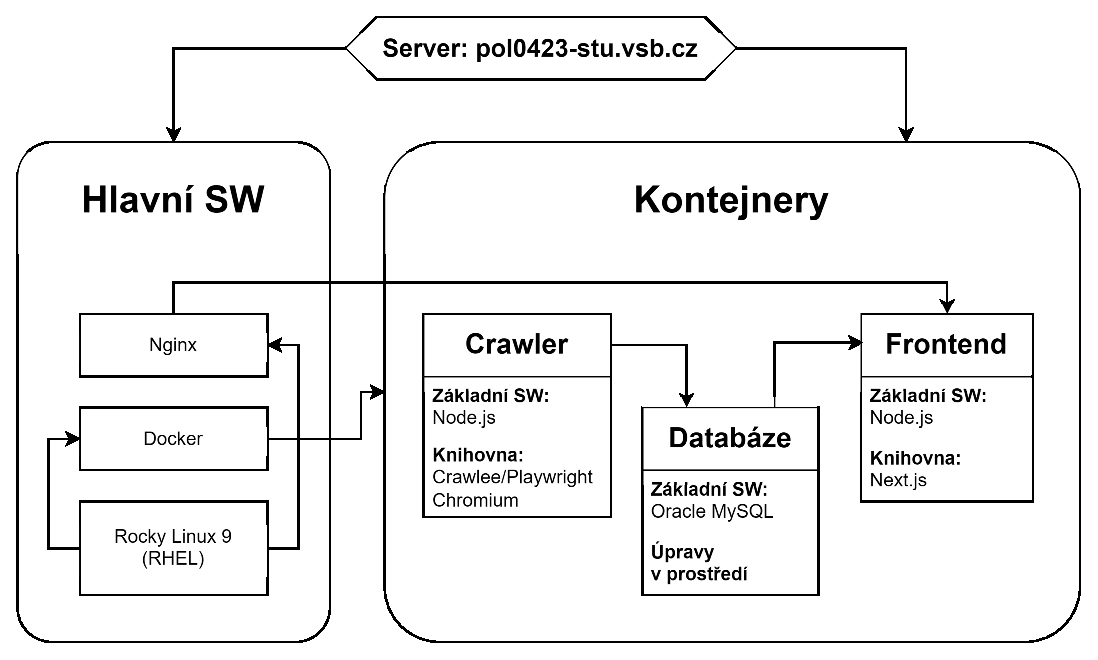
\includegraphics[width=0.75\linewidth]{Figures/structure.eps}
    \caption{Návrhový diagram technického řešení aplikace}
    \label{fig:structure-diagram}
\end{figure}

Jak můžete vidět na~přiloženém diagramu
v~obrázku~\ref{fig:structure-diagram}, návrh technického řešení
je~rozdělen na~hlavní software a~kontejnerovou část, která obsahuje
3~kontejnery. Crawler a~databáze jsou součástí backendu, který je~pomocí
databáze propojen s~frontendem.

Hlavním softwarem je~operační systém \emph{Linux}, na~němž běží
kontejnerizační SW \emph{Docker} a~dále webserverový SW \emph{Nginx}.
Docker poskytuje prostředí pro 3~kontejnerizované služby:

\begin{itemize}
    \item \textbf{Crawler:} Aktivní část backendu, která periodicky
        prohledává weby čerpacích stanic a~zjišťuje aktuální ceny
        pohonných hmot, které následně zapisuje do~databáze.
    \item \textbf{Databáze:} pasivní část backendu, která uchovává
        zaznamenané informace o~PHM (typ, kvalita, název, cena)
        daných ČS.
    \item \textbf{Frontend:} Uživatelské prostředí aplikace, které
        zprostředkovává uživateli grafické rozhraní, ve~kterém může
        vyhledávat, řadit a~filtrovat PHM a~jejich ceny na~základě
        geografické lokace a~maximálního okruhu.
\end{itemize}

Webservový SW Nginx poskytuje reverse proxy pro~snadný přístup ke~službě
prostým zadáním domény do~adresního řádku prohlížeče. Zamýšlené je~použití
SSL pro~HTTPS a~přesměrování nezabezpečeného portu HTTP na~zabezpečený port
HTTPS.

\section{Příprava operačního systému a konfigurace DNS}
\label{sec:os-preps-dns-config}

Jako operační systém serveru jsem zvolil Rocky Linux,
který mi byl~doporučen administrátory školní sítě. Tato linuxová
distribuce je~založena na~RHEL. Součástí konfigurace VM je~také
nastavení sítě. Neměnná IP adresa je~získána z~DHCP serveru,
avšak se~jedná pouze o~IPv4. IPv6 je~potřeba nastavit ručně.
Pro~server je~předkonfigurovaný také DNS záznam pro~IPv4 a~IPv6,
který vypadá následovně:

\begin{verbatim}
Name                       Type   TTL   Section    IPAddress
----                       ----   ---   -------    ---------
pol0423-stu.vsb.cz         AAAA   7200  Answer     2001:718:1001:207::64
pol0423-stu.vsb.cz         A      7200  Answer     158.196.109.64
\end{verbatim}

DNS záznam AAAA je~vazba na~IPv6 adresu, zatímco DNS záznam A
je~vazba na~IPv4.

\subsection{Instalace OS a počáteční konfigurace sítě serveru}
\label{sec:os-installation-initial-server-network-config}

Server se~nachází na~VMware vSphere serveru, dostupný
na~adrese vcs.vsb.cz. Prvním krokem byla instalace OS Rocky Linux,
která proběhla přes virtuální konzoli serveru. Instalační program
byl~ve~formě GUI, přes které jsem nastavil uživatelský účet správce
\texttt{marpolda}, nastavil jsem mu heslo a~zapnul mu práva správce.
Účet správce \texttt{root} je~vypnutý, lze~ho tedy použít jen pomocí
příkazu \texttt{sudo}. Po~instalaci OS byla dalším krokem instalace
nástrojů virtuálního stroje. Po~neúspěšném pokusu v~instalaci balíčku
VMware Tools jsem se~rozhodl využít místo toho otevřený balíček
\texttt{open-vm-tools}. Pro~práci s~textovými soubory jsem~si
také nainstaloval balíček \texttt{nano}, který poskytuje jednoduchý
textový editor přímo v~příkazovém řádku.

Dalším krokem je~nastavení IPv6 sítě. Jelikož IPv6 adresa není
DHCP serverem přidělena, je~potřeba adresu nastavit ručně. Pro~to
využijeme výše zmíněný DNS záznam pro~IPv6 vazbu. Tento proces
je~také zapotřebí provést pomocí virtuální konzole
(viz~listing~\ref{lst:net-modify} na~straně~\pageref{lst:net-modify}).

Otestujeme konektivitu IPv4 a~IPv6:

\begin{verbatim}
PS C:\Users\marpo> ping -4 pol0423-stu.vsb.cz

Pinging pol0423-stu.vsb.cz [158.196.109.64] with 32 bytes of data:
Reply from 158.196.109.64: bytes=32 time<1ms TTL=61
Reply from 158.196.109.64: bytes=32 time<1ms TTL=61
Reply from 158.196.109.64: bytes=32 time<1ms TTL=61
Reply from 158.196.109.64: bytes=32 time<1ms TTL=61

Ping statistics for 158.196.109.64:
    Packets: Sent = 4, Received = 4, Lost = 0 (0% loss),
Approximate round trip times in milli-seconds:
    Minimum = 0ms, Maximum = 0ms, Average = 0ms
PS C:\Users\marpo> ping -6 pol0423-stu.vsb.cz

Pinging pol0423-stu.vsb.cz [2001:718:1001:207::64] with 32 bytes of data:
Reply from 2001:718:1001:207::64: time=2ms
Reply from 2001:718:1001:207::64: time=1ms
Reply from 2001:718:1001:207::64: time<1ms
Reply from 2001:718:1001:207::64: time=1ms

Ping statistics for 2001:718:1001:207::64:
    Packets: Sent = 4, Received = 4, Lost = 0 (0% loss),
Approximate round trip times in milli-seconds:
    Minimum = 0ms, Maximum = 2ms, Average = 1ms
\end{verbatim}

Pro~přístup na~server pomocí SSH jsem~si také importoval ručně
přes konzoli SSH klíče obou mých počítačů, které využívají kvantově
rezistentní algoritmus \texttt{ed25519}. Z~důvodu bezpečnosti jsem
také provedl vypnutí přihlašování pomocí uživatelského hesla.
Tento krok jsem provedl vytvořením nového souboru
\texttt{/etc/ssh/sshd\_config.d/01-nopasswordlogin.conf}
s~následujícím obsahem:

\newpage

\begin{verbatim}
#################################################
# Disable password logins
#################################################

PasswordAuthentication no
\end{verbatim}

Veškeré soubory v~adresáři \texttt{/etc/ssh/sshd\_config.d} jsou
automaticky importovány v~souboru \texttt{/etc/ssh/sshd\_config},
který obsahuje konfiguraci SSH Daemon serveru.

Následně stačilo restartovat službu SSH Daemon:

\begin{verbatim}
# systemctl restart sshd.service
\end{verbatim}

Přístup na~server pomocí SSH jsem následně otestoval:
\begin{verbatim}
PS C:\Users\marpo> ssh marpolda@pol0423-stu.vsb.cz
The authenticity of host 'pol0423-stu.vsb.cz (158.196.109.64)' can't be established.
ED25519 key fingerprint is SHA256:oHy0UKZisrWxLKQtp5Xpezo53FNXZudKJ6/WVHeScI4.
This host key is known by the following other names/addresses:
    ~/.ssh/known_hosts:18: 158.196.109.64
Are you sure you want to continue connecting (yes/no/[fingerprint])? yes
Warning: Permanently added 'pol0423-stu.vsb.cz' (ED25519) to the list of known hosts.
Enter passphrase for key 'C:\Users\marpo/.ssh/id_ed25519':
Last login: Sat Mar  1 14:01:55 2025 from 158.196.52.150
[marpolda@pol0423-stu ~]$
\end{verbatim}

Z~mého druhého počítače jsem~se také úspěšně přihlásil:
\begin{verbatim}
[marpolda@archlinuxx-laptop ~]$ ssh pol0423-stu.vsb.cz
Enter passphrase for key '/home/marpolda/.ssh/id_ed25519':
Last login: Sun Mar  2 19:21:04 2025 from 2001:718:1001:698:99e2:f1ff:4e67:7618
[marpolda@pol0423-stu ~]$
\end{verbatim}

\section{Příprava kontejnerizace a~instalace služeb}
\label{sec:containers-preps-services-install}

Nyní, když máme nastavený základní přístup, můžeme přistoupit
k~instalaci softwaru pro~kontejnerizaci a~samotných kontejnerů
potřebných služeb. Pro~kontejnerizaci jsem~si vybral Docker,
který jsem nainstaloval z~příslušného balíčku následovně:

\begin{verbatim}
# dnf install docker
\end{verbatim}

Dalším krokem je~příprava samotných součástí aplikace. K~tomu
jsem~si vytvořil vývojové prostředí Gitu, ve~kterém bude
probíhat vývoj aplikace a~příprava pro~její nasazení na~server.
Toto prostředí se~také nachází na~GitHubu, kde~je~vidět
aktuální podoba této aplikace. Aplikaci jsem~se rozhodl pojmenovat
\emph{PetrolScan}. Všechny součásti aplikace obsahují soubor
\texttt{Dockerfile}, který vytváří Docker obrázek dané součásti.
Všechny tyto součásti jsou pospojovány souborem \texttt{docker-compose.yml},
který součásti propojuje a~vytváří tak ucelenou službu.

Vyvíjené součásti aplikace jsou:

\begin{itemize}
    \item Webová aplikace:
        \texttt{\url{https://github.com/POL0423/petrolscan-web-app}}
    \item Crawler:
        \texttt{\url{https://github.com/POL0423/petrolscan-crawler}}
    \item Docker Compose:
        \texttt{\url{https://github.com/POL0423/petrolscan-docker-compose}},
        Listing~\ref{src:docker-compose.yml}
        na~straně~\pageref{src:docker-compose.yml}
\end{itemize}

Veškeré zdrojové kódy lzeťaké nalézt v~datové příloze práce. GitHub
repozitáře jsou aktuální.

\subsection{Výběr softwaru pro~crawler}
\label{sec:crawler-solutions}

Jako první jsem~se rozhodl najít vhodné self-hosted webové crawlery
a~scrapery. Crawlerům se~v~teorii věnuji v~sekci~\ref{sec:research-crawlers}
v~kapitole~\ref{ch:initial-research} (Technologie pro~návrh webových aplikací)
na~straně~\pageref{sec:research-crawlers}. Na~dotaz k~vyhledávání
mi~ChatGPT \cite{givNscvAOqB1nMpq} %Ref: GPTCrawlers
našel následující možnosti:

\begin{itemize}
    \item Crawlee
    \item Scrapy
    \item EasySpider
\end{itemize}

Rozhodl jsem~se pro~Crawlee.

\subsubsection{Zkouška Crawlee}
\label{sec:crawlee-trial}

Tento crawler funguje v~Node.js, a~nabízí jednoduchou instalaci pomocí
jednoduchého příkazu. Crawler simuluje procházení webu člověkem pomocí
bezhlavičkových webových prohlížečů, které jsou schopné také interpretovat
Javascriptový kód.

Zkušební test ukázkového crawleru proběhl v~pořádku.
První pokus o~spuštění neuspěl, neboť chyběly Playwright bezhlavičkové
prohlížeče. Po~instalaci těchto prohlížečů se~již crawler spustil.

Velmi příjemným zjištěním bylo, že~builder již automaticky vygeneruje
soubor \texttt{Dockerfile}, pro~crawler tak lze~rovnou vytvořit
Docker image, který se~jen posléze nahraje na~Docker Hub a~lze s~ním
dále pracovat.

\subsubsection{Tvorba crawleru}
\label{sec:crawler-preps}

Nejprve je~nutné prozkoumat webové stránky různých čerpacích stanic.
Uvažujme tak tyto čerpací stanice:

\begin{itemize}
    \item \textbf{Globus}
    \item Orlen
    \item Shell
    \item EuroOil
    \item \textbf{ONO}
    \item MOL
    \item OMV
    \item Prim
    \item Makro
\end{itemize}

Pro~všechny tyto ČS tak je~nutné prozkoumat a~analyzovat jejich webové
stránky, abychom mohli z~daných webových stránek vytáhnout příslušná data.
Začíná mravenčí práce, a~sice prozkoumávání a~analýza skladby jednotlivých
webových stránek ČS, zápis struktury každého webu a~sestavení jednotlivých
šablon pro~náš crawler tak, aby byl~crawler schopen stránky procházet
a~získávat daný obsah. Crawler tato data z~webových stránek čte a~zaznamenává
do~databáze strukturovaně podle typu jednotlivých PHM, jejich značce
a~umístění ČS.

\subsubsection{Globus}
\label{sec:preps-globus}

Tato ČS patří velkoobchodnímu řetězci (hypermarketu) stejného jména
a~nachází se~výhradně vždy v~blízkosti prodejny. Globus lze~v~době
psaní této bakalářské práce najít jen v~16 různých městech a~městských
částí v~ČR:

\begin{itemize}
    \item Brno
    \item České Budějovice
    \item Chomutov
    \item Havířov
    \item Karlovy Vary ‒ Jenišov
    \item Liberec
    \item Olomouc
    \item Opava
    \item Ostrava
    \item Pardubice
    \item Plzeň ‒ Chotíkov
    \item Praha
    \begin{itemize}
        \item Čakovice
        \item Černý Most
        \item Štěrboholy
        \item Zličín
    \end{itemize}
    \item Trmice
\end{itemize}

Postup pro~získání informací o~cenách PHM z~ČS je následující.

\begin{enumerate}
    \item Na~webové stránce \url{www.globus.cz} klikneme na~tlačítko s~ikonou
        špendlíku. Pokud se~nás web zeptá na~výběr prodejny, zvolíme
        dle~požadavků (například Ostravu). Pokud je~zvolená prodejna
        nesprávná, lze výběr změnit kliknutím na~tlačítko „Změnit“
        v~prvním sloupci pop-up okénka.
    \item Požadované informace z~této ČS jsou ve~třetím sloupci (viz
        screenshot na~obrázku \ref{fig:globus-cs} na~stránce
        \pageref{fig:globus-cs}).
\end{enumerate}

Tento postup je~potřeba automatizovat. K~tomu nám právě poslouží již
zmíněný crawler. Každá ČS má~jinou strukturu webu, a~proto je~potřeba
vytvořit pro~každý web jeho vlastní crawler.

\subsubsection{ONO}
\label{sec:preps-ono}

ČS~ONO jsou v~samostatné síti ČS provozované společností Tank ONO s.r.o.
Web se~nachází na~adrese \url{www.tank-ono.cz}, který je~velmi jednoduchý
a~přehledný. Postup k~získání informací z~ČS je následující:

\begin{enumerate}
    \item Načteme hlavní webovou stránku \url{www.tank-ono.cz}. Zobrazí~se
        nám mapa s~jednotlivými pobočkami sítě ČS~ONO. Na~této webové
        stránce se~nachází celkem 43~stanic. Jejich mapu lze~vidět
        na~obrázku~\ref{fig:tank-ono-mapa}
        na~straně~\pageref{fig:tank-ono-mapa}.
        V~tabulce~\ref{tab:tank-ono-pobocky}
        na~straně~\pageref{tab:tank-ono-pobocky} lze~vidět jejich výčet.
    \item Kliknutím na~jednu z~položek v~seznamu nebo kliknutím na~pozici
        na~mapě si~lze zobrazit detail konkrétní ČS.
        Na~obrázku~\ref{fig:tank-ono-stranka}
        na~straně~\pageref{fig:tank-ono-stranka} lze vidět strukturu webové
        stránky detailu ČS. Vlevo nahoře~(a) je~název a~umístění ČS, zatímco
        vpravo dole je~vidět tabulka PHM~(b) včetně jejich cen v~Kč~(c)
        a~eurech. Toto jsou data, která nás zajímají.
\end{enumerate}

\begin{table}[h]
    \centering
    \caption{Seznam ČS ONO}
    \label{tab:tank-ono-pobocky}
    \begin{tabular}{r l|r l}
        1.    & ČS Plzeň, Domažlická        & 24.   & ČS Sukorady u~Mladé
                                                        Boleslavi\\
        2.    & ČS Nýřany                   & 25.   & ČS Podolí u~Písku\\
        3.    & ČS Plzeň, Studentská        & 26.   & ČS Planá nad~Lužnicí\\
        4.    & ČS Sokolov                  & 27.   & ČS Spytihněv\\
        5.    & ČS Teplice                  & 28.   & ČS Mošnov\\
        6.    & ČS Cheb                     & 29.   & ČS Kojetice-Tůmovka\\
        7.    & ČS Milovice u~Hořic         & 30.   & ČS Cvikov\\
        8.    & ČS Chlumec                  & 31.   & ČS Chomutov – Přečaply\\
        9.    & ČS Jihlava                  & 32.   & ČS Zádveřice u~Zlína\\
        10.   & ČS Trutnov                  & 33.   & ČS Brno-Popovice\\
        11.   & ČS Jindřichův Hradec        & 34.   & ČS Roudnice nad~Labem\\
        12.   & ČS Vysoké Mýto              & 35.   & ČS Vysokov u~Náchoda\\
        13.   & ČS Havraň                   & 36.   & ČS Praha – Štěrboholy\\
        14.   & ČS Kolaje u~Poděbrad        & 37.   & ČS Řasnice-Strážný\\
        15.   & ČS Ústí n. L., Božtěšická   & 38.   & ČS Břest u~Kroměříže\\
        16.   & ČS Praha, Dolní Měcholupy   & 39.   & ČS Vojtanov\\
        17.   & ČS Kbelnice                 & 40.   & ČS Dobkovice u~Děčína\\
        18.   & ČS Havlovice u~Domažlic     & 41.   & ČS Březno u~Loun D7\\
        19.   & ČS Mělník                   & 42.   & ČS Brno-Hviezdoslavova\\
        20.   & ČS Krupá u~Rakovníka        & 43.   & ČS Studénka – D1
                                                        exit 336\\
        21.   & ČS Dolní Dvořiště – ONO I   & 44.   & ČS Ostrov nad Ohří\\
        22.   & ČS Dolní Dvořiště – ONO II  & 45.   & ČS Chlumčany u~Přeštic\\
        23.   & ČS Církvice u~Kutné Hory
    \end{tabular}
\end{table}

\subsubsection{Vyřazené čerpací stanice}
\label{sec:preps-removed-stations}

Během analýzy zmíněných webů ČS jsem zjistil, že~právě pouze z~webů
Globus a~ONO jsou použitelné ceny PHM. Následující weby řetězců ČS
jsem musel z~projektu vyřadit, neboť nesplňují požadavky k~dolování dat.

\begin{itemize}
    \item \textbf{OMV:} Tato síť ČS poskytuje ceny PHM ve~formátu,
        který vyžaduje použití OCR čtečky, jejíž implementace
        by~byla velmi náročná, a~časově by~nebylo reálné čtečku
        do~projektu zakomponovat.
    \item \textbf{Orlen:} Webové stránky této ČS využívají REST API,
        což je~vysoké plus. Ale~to samo o~sobě nestačí. Pokud ani
        v~API, ani na~webové stránce nejsou k~dispozici ceny PHM,
        jen slevy na~tankovací kartu či~aplikaci této sítě, nelze
        tato data v~porovnání cen PHM použít.
    \item \textbf{Shell, EuroOil, MOL a Prim:} Tyto ČS informace
        o~cenách PHM na~svých webových stránkách vůbec neposkytují,
        čímž nelze data z~těchto webových stránek použít.
    \item \textbf{Makro:} Tato ČS sice ceny na~webu uvádí, a to
        v~přijatelném formátu, ale~web implementuje pokročilé
        antiscraping mechanismy, které detekují a~blokují crawlery
        podobné tomuto projektu. Z~toho důvodu byl tento crawler
        během jeho vývoje vyřazen. Crawler zkrátka nemohl tyto
        mechanismy obejít a~k~implementaci protichůdných opatření
        již nezbýval dostatek času.
\end{itemize}

Po~konzultaci s~vedoucím bakalářské práce jsme dospěli k~závěru,
že~pro~demonstraci funkčnosti mého návrhu je~ověření na~dvou sítích ČS
dostatečné, celý projekt je~veřejně dostupný pod licencí MIT na~GitHubu
a~práce může~být v~budoucnu rozšířena o~další stanice PHM.

\subsubsection{Návrh strukturizace crawleru}
\label{sec:preps-crawler-structure}

Pro~snazší vývoj a~lepší údržbu aplikace je~potřeba ji~rozdělit na~jednotlivé
části, které plní své~specifické úlohy.

\begin{itemize}
    \item \textbf{Hlavní část:} Jedná~se o~hlavní spouštěcí kód, který volá
        další moduly.
    \item \textbf{Dílčí crawlery:} Tyto části provádějí samotnou sklizeň.
        Jedná~se o~samotnou implementaci logiky dílčích crawlerů. To~jsou
        dva moduly: Globus a~ONO. Oba tyto moduly mají společný nadřazený
        abstraktní modul, který definuje společné vlastnosti a~metody
        těchto modulů.
    \item \textbf{Databázová spojka:} Tato část propojuje crawlery s~databází
        a~umožňuje jim do~databáze zapisovat nasbíraná data.
    \item \textbf{Definice datových typů:} V~této části definuji některé
        datové typy, které dílčí crawlery používají. Datové typy jsou
        definovány kvůli snadnější identifikaci a~implementaci práce
        s~informacemi.
    \item \textbf{Crontab:} Jedná se o~skript, který periodicky každý den
        ve~3:00 spouští crawler a~zajišťuje zapisování výstupu konzole
        do~logovacího souboru.
\end{itemize}

\subsection{Databáze}
\label{sec:preps-db}

Databázím se~podrobně věnuji v~teoretickém rozboru
v~sekci~\ref{sec:research-db} kapitoly~\ref{ch:initial-research}
na~straně\pageref{sec:research-db}.

Pokud je~crawler mozkem aplikace, který vyhledává data a~ukládá~je,
pak~databáze je~určitě srdcem celé aplikace, protože umožňuje její fungování.
Bez~databáze by~aplikace fungovat nemohla. K~dispozici je~několik různých
softwarů. Především bych vyjmenoval následující možnosti:

\begin{itemize}
    \item \textbf{MySQL:} Zřejmě nejpoužívanější databázový software na~světě.
        Jeho předností je~jednoduché použití, všestrannost a~široká
        kompatibilita s~různými softwary pro~backend i~frontend. MySQL
        je~k~dispozici ve~více variantách:
        \begin{enumerate}
            \item \textbf{MySQL:} Originální verze MySQL, která je~stále
                aktivně vyvíjená. Tuto verzi lze~najít na~většině komerčních
                serverů. Dnes vlastněná společností Oracle.
            \item \textbf{MariaDB:} Jedná~se o~fork originální verze MySQL
                (fork znamená, že~se~jedná o~verzi odvozenou z~původní).
                V~dnešní době pro~většinu menších projektů příjemná
                alternativa, která je~zdarma a~open-source.
        \end{enumerate}
    \item \textbf{PostgreSQL:} Rychlý a~moderní nástupce MySQL. Tento
        databázový engine je~nejvíce kompatibilní s~moderními nástupci
        webové technologie (zejména Reactu, viz~další podsekce), které
        v~současnosti dominují internetu.
    \item \textbf{SQLite:} Jednoduchý a~nenáročný databázový model určený
        pro~lokální aplikace malé velikosti. Předností tohoto modelu
        je~skutečnost, že~běží přímo v~dané aplikaci a~nepotřebuje tedy
        zvlášť server pro~správu dat. Nevýhodou je~malá škálovatelnost.
\end{itemize}

Pro~svou aplikaci jsem~si vybral \textbf{MySQL}, jelikož poskytuje širokou
kompatibilitu, je~jednoduchý k~použití, všestranný a~mám s~ním již předchozí
zkušenost. Jedná se o~průkopníka v~moderních databázových systémech, který
vydláždil cestu jeho nástupcům. MySQL používá SQL pro~komunikaci s~aplikací,
což je~strukturovaný dotazovací jazyk nápadně podobný angličtině.

\subsection{Frontend}
\label{sec:preps-frontend}

Podrobně se~frontendům věnuji v~teoretickém rozboru
v~sekci~\ref{sec:research-frontend} kapitoly~\ref{ch:initial-research}.
%na~straně~\pageref{sec:research-frontend}.

Frontend je~tváří celé aplikace. Jedná se o~tu~část aplikace, kterou vidí
její uživatel. Tato část zpracovává data z~databáze a~zprostředkovává je
uživateli pro~jeho další zpracování. Existuje mnoho webových technologií
založených na~různých programovacích a~značkovacích jazycích, které jsou
na~internetu široce používané. Vyjmenoval bych zejména tyto nejpoužívanější:

\begin{itemize}
    \item \textbf{Statické HTML/CSS:} Jedná~se čistě o~statické webové
        stránky, tak jak jsou uložené na~webovém serveru. Jednoduchým
        HTTP requestem si~uživatel prostřednictvím webového prohlížeče
        zažádá o~stránku, webový server najde její odpovídající soubor,
        a~obsah stránky zašle do~počítače uživatele. Výhoda je~extrémní
        jednoduchost, nevýhodou~je, že~nelze vytvářet složitější aplikace,
        které vyžadují určitou interaktivitu a~případně nějaké složitější
        výpočty. Jedná~se o~první webovou technologii.
    \item \textbf{HTML/CSS s JS:} Malý upgrade z~předchozí technologie,
        nyní obohacená o~jednoduchou formu programování na~webu. JavaScript
        nabízí možnosti, jak stránku doplnit o~různé efekty a~interaktivitu,
        a~umožňuje jednoduché algoritmizační úkony. Výhodou je~jednoduchost
        a~jistá forma interaktivizace. Nevýhodou je~fakt, že~veškerý
        programový kód aplikace běží v~počítači uživatele, a~tak není možné
        pracovat s~databází na~serveru, aniž by~došlo k~úniku autentizačních
        údajů.
    \item \textbf{PHP:} Jedná se o~doplňkový software v~současnosti nejvíce
        využívaný společně s~webovým serverem Apache či~Nginx, a~zároveň
        se~jedná o~programovací jazyk, ve~kterém jsou psané webové aplikace.
        PHP může sloužit zároveň jako backend i~frontend. Uživateli tento
        software posílá data nejčastěji ve~formátu HTML/CSS/JS, ale~může
        využívat i~některé formáty serializovaných dat (např. XML nebo JSON),
        případně obrázkové, video či~audio formáty. Výhodou je~skutečnost,
        že~tento software umožňuje část aplikace spouštět na~serveru
        a~uživatel tak uvidí konečný výstup, případně částečně zpracovaný
        výstup, se~kterým lze~posléze manipulovat na~uživatelské straně.
        Nevýhodou je~poměrně složitější a~obtížnější serializace dat, která
        je~způsobená zejména stářím standardu. V~PHP existuje několik
        frameworků, ale~jen jeden nejpoužívanější framework je~univerzální
        pro~širokou škálu různých projektů, které vyžadují vývoj vlastních
        funkcí: \textbf{Laravel}. Tento framework umožňuje tvorbu originální
        webové aplikace v~PHP, kde jsou k~dispozici vývojářské nástroje
        pro~správu dat, jejich čtení, zápis a~další zpracování. Nevýhodou
        tohoto frameworku jsou chybějící nástroje pro~rychlý webdesign.
        Na~druhou stranu však má~vývojář volnou ruku ve~volbě vlastního
        řešení.
    \item \textbf{Node.js:} Node.js lze úspěšně použít nejen pro~backend,
        ale~také i~pro~frontend. V~kombinaci s~dalšími frameworky, které
        umožňují jednodušší tvorbu webové aplikace, se~jedná o~moderní
        způsob poskytování webového obsahu. Toto jsou nejpoužívanější
        frameworky:

        \begin{itemize}
            \item \textbf{React:} Základní průkopník moderního webu.
                Jedná~se o~knihovnu, která položila základy moderního
                webu a~vytvořila koncept webového serveru v~JavaScriptu.
            \item \textbf{Next.js:} Moderní React framework vyvíjený
                společností Vercel. Výhodou je~jednoduchost použití
                a~nativní inkluze moderních CSS frameworků, jako např.
                Tailwind CSS nebo CSS Modules.
            \item \textbf{Vue.js:} Konkurenční framework oproti Reactu.
                Jedná se o~progresivní framework, který poskytuje jednoduché
                vývojářské nástroje pro~frontend.
            \item \textbf{Nuxt.js:} Odvozený z~Vue.js, doplňuje jej
                o~full-stack nástroje, lze jej tedy využít i~jako backend.
        \end{itemize}
\end{itemize}

Pro~mou aplikaci jsem~se rozhodl využít Node.js s~využitím frameworku Next.js.
S~Node.js již mám nějaké předchozí zkušenosti, JavaScript je~poměrně
jednoduchý programovací jazyk, z~něj odvozený TypeScript navíc přidává
jednoduché zabezpečení aplikace z~hlediska datových typů. Next.js se~mi~jeví
jako optimální volba, vzhledem k~jednoduchosti a~dostupnosti různých
předpřipravených nástrojů pro~rychlý webový design.

\endinput
